\documentclass[tikz, border=10pt]{standalone}
\usepackage{tikz}
\usepackage{amsmath}
\usetikzlibrary{arrows.meta, positioning, backgrounds, fit}

\definecolor{obscolor}{RGB}{214,229,252}
\definecolor{traincolor}{RGB}{255,213,170}
\definecolor{outcolor}{RGB}{200,240,200}
\definecolor{trainborder}{RGB}{210,70,40}
\definecolor{panelbg}{RGB}{248,248,248}
\definecolor{deploycolor}{RGB}{232,245,232}
\definecolor{deployborder}{RGB}{60,140,60}

\begin{document}
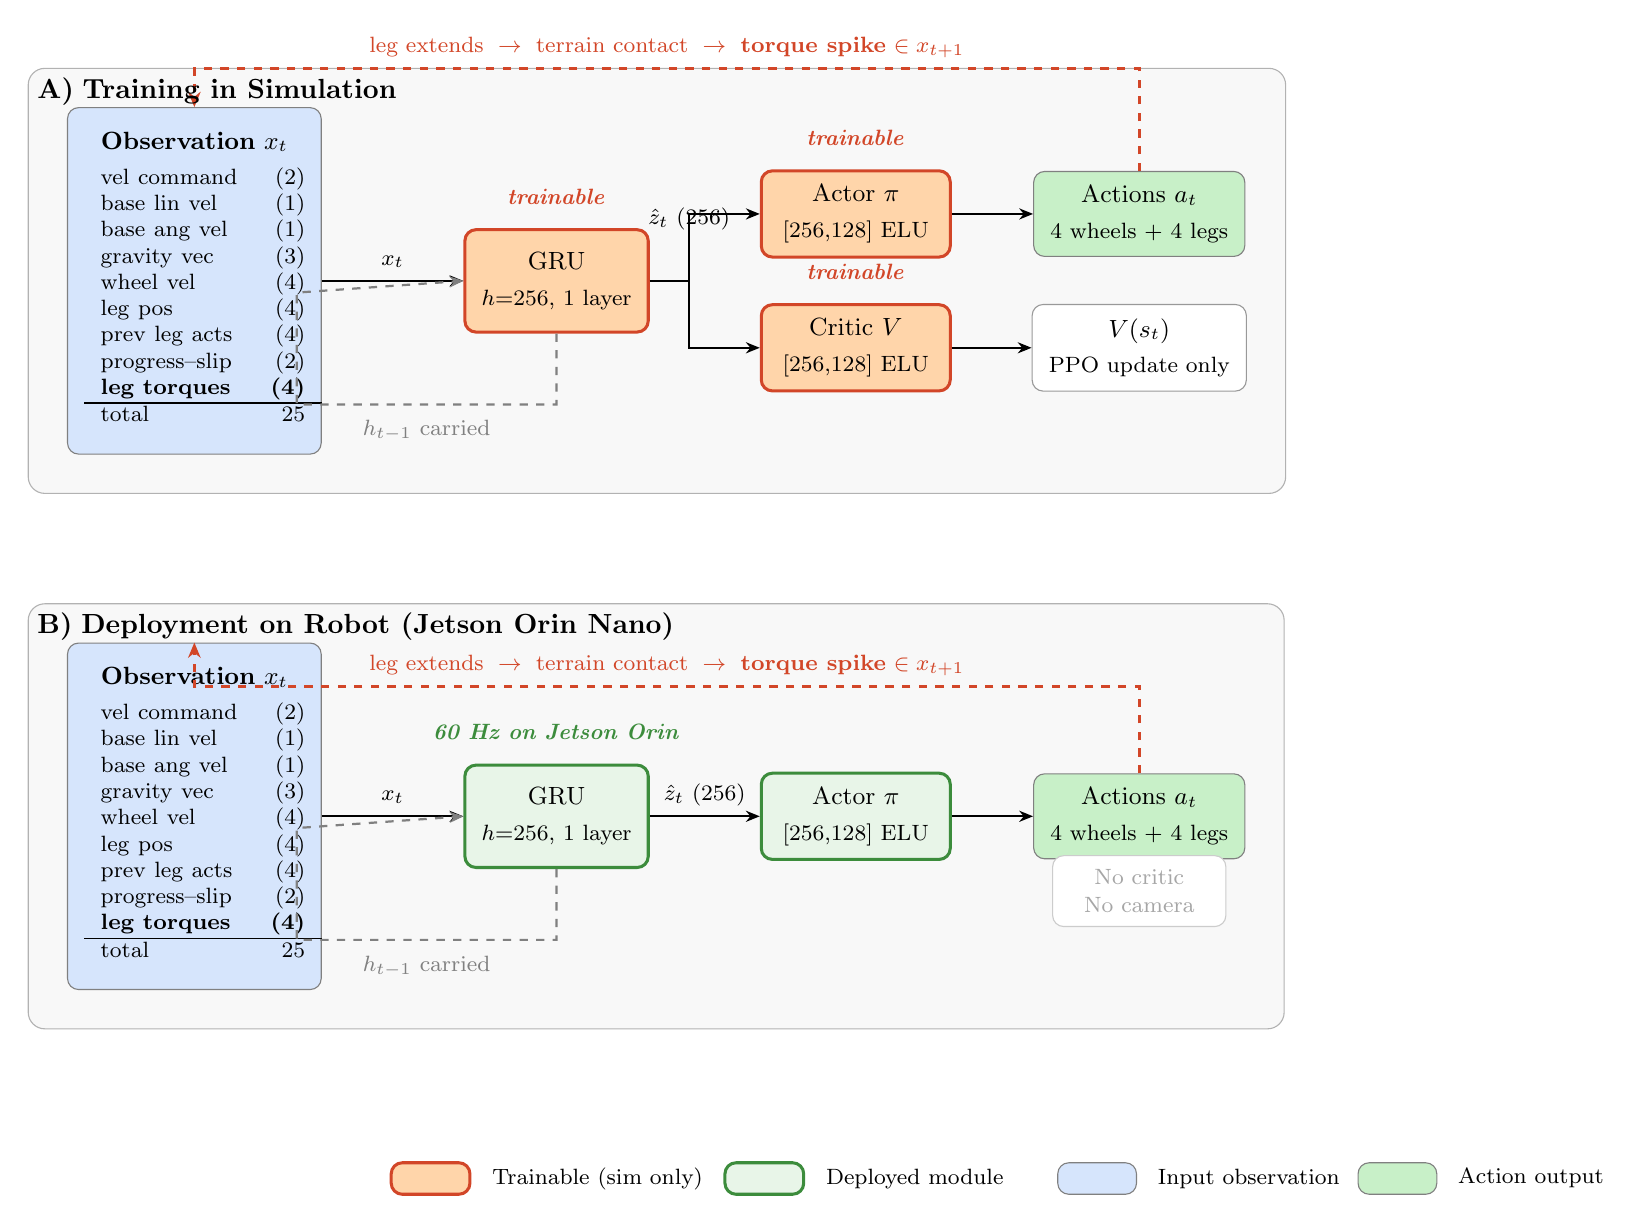
\begin{tikzpicture}[
    every node/.style={font=\small},
    box/.style={draw, rounded corners=4pt, align=center,
                inner xsep=6pt, inner ysep=5pt},
    obsbox/.style={box, fill=obscolor, draw=black!50},
    trainbox/.style={box, fill=traincolor, draw=trainborder, line width=1.1pt},
    outbox/.style={box, fill=outcolor, draw=black!50},
    plainbox/.style={box, fill=white, draw=black!40},
    deploybox/.style={box, fill=deploycolor, draw=deployborder, line width=1.1pt},
    arr/.style={-{Stealth[length=5pt,width=4pt]}, thick},
    darr/.style={-{Stealth[length=5pt,width=4pt]}, thick, dashed, gray},
    probarr/.style={-{Stealth[length=5.5pt,width=4.5pt]}, line width=1.2pt,
                    color=trainborder, dashed},
]

%% =========================================================
%% PANEL A — Training in Simulation  (y baseline = 0)
%% =========================================================

%% --- Observation ---
\node[obsbox, minimum width=3.0cm, minimum height=4.4cm, text width=2.8cm]
  (obs) at (0, 0)
  {\textbf{Observation} $x_t$\\[4pt]
   \footnotesize
   \begin{tabular}{lr}
     vel command   & (2)  \\
     base lin vel  & (1)  \\
     base ang vel  & (1)  \\
     gravity vec   & (3)  \\
     wheel vel     & (4)  \\
     leg pos       & (4)  \\
     prev leg acts & (4)  \\
     progress--slip& (2)  \\
     \textbf{leg torques} & \textbf{(4)}\\
     \hline
     total         & 25
   \end{tabular}
  };

%% --- GRU ---
\node[trainbox, minimum width=2.2cm, minimum height=1.3cm]
  (lstm) at (4.6, 0)
  {GRU\\[2pt]\footnotesize $h{=}256$, 1 layer};

%% --- Actor ---
\node[trainbox, minimum width=2.4cm, minimum height=0.9cm]
  (actor) at (8.4, 0.85)
  {Actor $\pi$\\[2pt]\footnotesize [256,128] ELU};

%% --- Critic ---
\node[trainbox, minimum width=2.4cm, minimum height=0.9cm]
  (critic) at (8.4, -0.85)
  {Critic $V$\\[2pt]\footnotesize [256,128] ELU};

%% --- Outputs ---
\node[outbox, minimum width=2.2cm, minimum height=0.9cm]
  (action) at (12.0, 0.85)
  {Actions $a_t$\\[2pt]\footnotesize 4 wheels + 4 legs};

\node[plainbox, minimum width=2.2cm, minimum height=0.9cm]
  (value) at (12.0, -0.85)
  {$V(s_t)$\\[2pt]\footnotesize PPO update only};

%% --- Forward arrows ---
\draw[arr] (obs.east)   -- node[above, yshift=1pt]{\footnotesize $x_t$} (lstm.west);
\draw[arr] (lstm.east)  -- ++(0.5,0) |- (actor.west)
           node[pos=0.3, above, font=\footnotesize]{$\hat{z}_t$ (256)};
\draw[arr] (lstm.east)  -- ++(0.5,0) |- (critic.west);
\draw[arr] (actor.east) -- (action.west);
\draw[arr] (critic.east)-- (value.west);

%% --- Hidden state loop (bottom) ---
\draw[darr]
  (lstm.south) -- ++(0,-0.9)
  -- node[below, yshift=-2pt, font=\footnotesize]{$h_{t-1}$ carried}
     ++(-3.3,0)
  -- ++(0, 1.42)
  -- (lstm.west);

%% --- Active probing loop (top) ---
\draw[probarr]
  (action.north) -- ++(0, 1.3)
  -- node[above, font=\footnotesize, align=center]
     {leg extends $\;\rightarrow\;$ terrain contact
      $\;\rightarrow\;$ \textbf{torque spike} $\in x_{t+1}$}
     ++(-12.0, 0)
  -- (obs.north);

%% --- Trainable labels ---
\node[font=\footnotesize\bfseries, color=trainborder, above=5pt of lstm]  {\textit{trainable}};
\node[font=\footnotesize\bfseries, color=trainborder, above=5pt of actor] {\textit{trainable}};
\node[font=\footnotesize\bfseries, color=trainborder, above=5pt of critic]{\textit{trainable}};

%% --- Panel A border + label ---
\begin{scope}[on background layer]
  \node[draw=black!30, fill=panelbg, rounded corners=6pt,
        fit=(obs)(lstm)(actor)(critic)(action)(value),
        inner sep=14pt] (panelA) {};
\end{scope}
\node[font=\normalsize\bfseries, anchor=north west] at (panelA.north west)
  {A)\;Training in Simulation};


%% =========================================================
%% PANEL B — Deployment on Robot  (shifted down)
%% =========================================================
\def\dy{-6.8}   % vertical offset for panel B

%% --- Observation (deployment) ---
\node[obsbox, minimum width=3.0cm, minimum height=4.4cm, text width=2.8cm]
  (dobs) at (0, \dy)
  {\textbf{Observation} $x_t$\\[4pt]
   \footnotesize
   \begin{tabular}{lr}
     vel command   & (2)  \\
     base lin vel  & (1)  \\
     base ang vel  & (1)  \\
     gravity vec   & (3)  \\
     wheel vel     & (4)  \\
     leg pos       & (4)  \\
     prev leg acts & (4)  \\
     progress--slip& (2)  \\
     \textbf{leg torques} & \textbf{(4)}\\
     \hline
     total         & 25
   \end{tabular}
  };

%% --- GRU (deployment) ---
\node[deploybox, minimum width=2.2cm, minimum height=1.3cm]
  (dlstm) at (4.6, \dy)
  {GRU\\[2pt]\footnotesize $h{=}256$, 1 layer};

%% --- Actor only ---
\node[deploybox, minimum width=2.4cm, minimum height=0.9cm]
  (dactor) at (8.4, \dy)
  {Actor $\pi$\\[2pt]\footnotesize [256,128] ELU};

%% --- Output ---
\node[outbox, minimum width=2.2cm, minimum height=0.9cm]
  (daction) at (12.0, \dy)
  {Actions $a_t$\\[2pt]\footnotesize 4 wheels + 4 legs};

%% --- No critic label ---
\node[plainbox, draw=black!20, fill=white!60, minimum width=2.2cm,
      minimum height=0.9cm, text=black!35]
  (nocritic) at (12.0, \dy - 0.95)
  {\footnotesize No critic\\[-1pt]\footnotesize No camera};

%% --- Forward arrows (deployment) ---
\draw[arr] (dobs.east)    -- node[above, yshift=1pt]{\footnotesize $x_t$} (dlstm.west);
\draw[arr] (dlstm.east)   -- node[above, font=\footnotesize]{$\hat{z}_t$ (256)} (dactor.west);
\draw[arr] (dactor.east)  -- (daction.west);

%% --- Hidden state loop (deployment, bottom) ---
\draw[darr]
  (dlstm.south) -- ++(0,-0.9)
  -- node[below, yshift=-2pt, font=\footnotesize]{$h_{t-1}$ carried}
     ++(-3.3,0)
  -- ++(0, 1.42)
  -- (dlstm.west);

%% --- Active probing loop (deployment, top) ---
\draw[probarr]
  (daction.north) -- ++(0, 1.1)
  -- node[above, font=\footnotesize, align=center]
     {leg extends $\;\rightarrow\;$ terrain contact
      $\;\rightarrow\;$ \textbf{torque spike} $\in x_{t+1}$}
     ++(-12.0,0)
  -- (dobs.north);

%% --- 60 Hz label ---
\node[font=\footnotesize\bfseries, color=deployborder, above=5pt of dlstm]
  {\textit{60 Hz on Jetson Orin}};

%% --- Panel B border + label ---
\begin{scope}[on background layer]
  \node[draw=black!30, fill=panelbg, rounded corners=6pt,
        fit=(dobs)(dlstm)(dactor)(daction)(nocritic),
        inner sep=14pt] (panelB) {};
\end{scope}
\node[font=\normalsize\bfseries, anchor=north west] at (panelB.north west)
  {B)\;Deployment on Robot (Jetson Orin Nano)};

%% =========================================================
%% LEGEND  (below panel B)
%% =========================================================
\def\legy{-11.4}
\node[trainbox, minimum width=1.0cm, minimum height=0.4cm] (l1) at (3.0, \legy) {};
\node[font=\footnotesize, right=4pt of l1] {Trainable (sim only)};

\node[deploybox, minimum width=1.0cm, minimum height=0.4cm,
      right=3.2cm of l1] (l2) {};
\node[font=\footnotesize, right=4pt of l2] {Deployed module};

\node[obsbox, minimum width=1.0cm, minimum height=0.4cm,
      right=3.2cm of l2] (l3) {};
\node[font=\footnotesize, right=4pt of l3] {Input observation};

\node[outbox, minimum width=1.0cm, minimum height=0.4cm,
      right=2.8cm of l3] (l4) {};
\node[font=\footnotesize, right=4pt of l4] {Action output};

\end{tikzpicture}
\end{document}
